\section{The Extended Role-Based Access Control Scheme}
\label{sec:hybrid.scheme}

To support security model handling in the extended \gls{rbac} model, we introduce a set of predicates, assign predicates to entities, add new queries, and redefine the entailment function. 

Predicates are defined by the administrator based on the needs of the company. To enable this, a new set of predicates \( \predicates \) was introduced, with each predicate being represented as a string. As a result, the state transition system is redefined by adding the set \( \predicates \), resulting in the system being represented as \( \angular{\states, \queries, \entailment, \scrules, \predicates} \). Predicates are applied to an entity (i.e., user, role, the \gls{csp}), and they are unary. A new set, \( \prassignement \), was introduced to store the assignment. \( \prassignement \) is defined as \( \prassignement \subseteq \predicates \times (\users \cup \roles \cup \files) \). Consequently, the state was extended to also contain the set \( \prassignement \), resulting in \( \angular{\users, \roles, \files, \urassignement, \frassignement, \prassignement} \). New queries have been added to the set of queries \( \queries \), on top of the already existing \( \canDoQ \) query. Each query adjusts a specific tunable aspect of the system, such as whether to encrypt a file or not, and whether to re-encrypt a file. \Cref{tab:hybrid_queries} describes the queries, which are not customizable by the administrator. The entailment function \( \entailment \) serves as the connection between company phenomenons (the predicates) and customizable features (the queries). It is necessary for the administrator to define the entailment function for new queries based on the chosen security model. 

Note that the administrator cannot modify the entailment function for the query \( \canDoQ \), as doing so would prevent the use of a centralized \gls{rbac} and \gls{cac} mechanism. Additionally, modifying the \( \canDoQ \) query would result in a model that is no longer \gls{rbac}.

\Cref{fig:exrbac_components} illustrates the predicates, queries, and entailment function, and distinguishes between the \erbac and the security model.

\Cref{sec:hybird_istantiation} contains an example of a realistic security model instantiation.

\begin{figure}[t!]
	\centering
	
	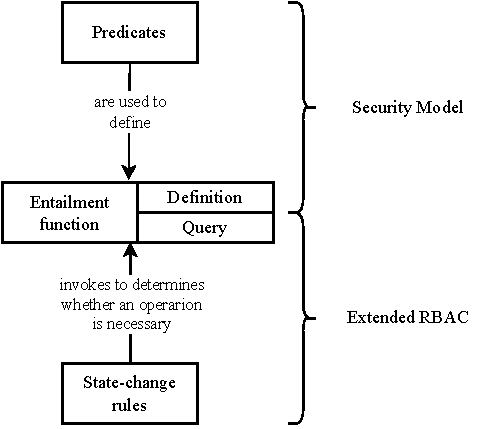
\includegraphics[width=0.5\textwidth]{assets/img2/security_model.pdf}
	
	\caption{The Interaction Between Components}
	\label{fig:exrbac_components}
\end{figure}


\wraptable{|l|X|}{\label{tab:hybrid_queries}The \( \queries \) of the hybrid model}{
	\twocols{\tabletitle{Query}}
	{\tabletitle{Description}}
	\twocols{\( \canDoQ \)}
	{Determines whether user \( \user \) has access to file \( \file \) to perform the action \( \operation \)}
	\twocols{\( \isEncryptionNeededQ \)}
	{Determines whether it is necessary to encrypt the file \( \file \)}
	\twocols{\( \isReencryptionNeededOnRPQ \)}
	{Determines whether it is necessary to re-encrypt the file \( \file \) when the permission \( \angular{\operation, \file} \) is revoked}
	\twocols{\( \isEagerReencNeededOnRPQ \)}
	{Determines whether it is necessary immediately to re-encrypt the file \( \file \) when the permission \( \angular{\operation, \file} \) is revoked}
	\twocols{\( \isRoleKeyRotationNeededOnRURQ \)}
	{Determines whether it is necessary to rotate the key of role \( \role \) when 
		the membership of the user \( \user \) to the role \( \role \) is revoked}
	\twocols{\( \isReencryptionNeededOnRURQ \)}
	{Determines whether it is necessary to re-encrypt the file \( \file \) when the membership of the user \( \user \) to the role \( \role \) is revoked}
	\twocols{\( \isEagerReencNeededOnRURQ \)}
	{Determines whether it is necessary to re-encrypt immediately the file \( \file \) when the membership of the user \( \user \) to the role \( \role \) is revoked}
}

\pagelisting{\label{list:extended_changestate}The state-change rules \( \scrules \) of the hybrid model }{\scriptsize}{b!}{
    \begin{itemize}

        %% --- addUser ---
        \item \( \addUserF \)
        \begin{itemize}
            \item Update state with \( \statete{\users \cup \setof{\user}}{\roles}{\files}{\urassignement}{\frassignement}{\prassignement} \)
            \item \( \addUserFC \)
            \item \( \addUserFK \)
        \end{itemize}

        %% --- deleteUser ---
        \item \( \deleteUserF \)
        \begin{itemize}
            \item Update state with \( \statete{\users \setminus \setof{\user}}{\roles}{\files}{\urassignement}{\frassignement}{\prassignement} \)
            \item For each \( (\user, \role) \in \urassignement \):
            \begin{itemize}
                \item \( \revokeUserFromRoleFC \)
                \item \( \revokeUserFromRoleFK \)
            \end{itemize}
            \item \( \deleteUserFC \)
            \item \( \deleteUserFK \)
        \end{itemize}

        %% --- addRole ---
        \item \( \addRoleF \)
        \begin{itemize}
            \item Update state with \( \statete{\users}{\roles \cup \setof{\role}}{\files}{\urassignement}{\frassignement}{\prassignement} \)
            \item \( \addRoleFC \)
            \item \( \addRoleFK \)
        \end{itemize}

        %% --- deleteRole ---
        \item \( \deleteRoleF \)
        \begin{itemize}
            \item Update state with \( \statete{\users}{\roles \setminus \setof{\role}}{\files}{\urassignement}{\frassignement}{\prassignement} \)
            \item For each \( (\role, \twoang{\operation}{\file}) \in \frassignement \):
            \begin{itemize}
                \item \( \revokePermissionFromRoleF \)
            \end{itemize}
            \item \( \deleteRoleFC \)
            \item \( \deleteRoleFK \)
        \end{itemize}

        %% --- addResource ---
        \item \( \addResourceF \)
        \begin{itemize}
            \item Update state with \( \statete{\users}{\roles}{\files \cup \setof{\file}}{\urassignement}{\frassignement}{\prassignement} \)
            \item \( \addResourceFC \)
        \end{itemize}

        %% --- deleteResource ---
        \item \( \deleteResourceF \)
        \begin{itemize}
            \item Update state with \( \statete{\users}{\roles}{\files \setminus \setof{\file}}{\urassignement}{\frassignement}{\prassignement} \)
            \item \( \deleteResourceFC \)
            \item For each \( (\role, \twoang{\operation}{\file}) \in \frassignement \):
            \begin{itemize}
                \item \( \revokePermissionFromRoleF \)
            \end{itemize}
            \item If \( \isEncryptionNeededF \):
            \begin{itemize}
                \item \( \deleteResourceFK \)
            \end{itemize}
        \end{itemize}

        %% --- assignUserToRole ---
        \item \( \assignUserToRoleF \)
        \begin{itemize}
            \item Update state with \( \statete{\users}{\roles}{\files}{\urassignement \cup \setof{(\user, \role)}}{\frassignement}{\prassignement} \)
            \item \( \assignUserToRoleFC \)
            \item \( \assignUserToRoleFK \)
        \end{itemize}

        %% --- assignPermissionToRole ---
        \item \( \assignPermissionToRoleF \)
        \begin{itemize}
            \item Update state with \( \statete{\users}{\roles}{\files}{\urassignement}{\frassignement \cup (\role, \twoang{\operation}{\file})}{\prassignement} \)
            \item \( \assignPermissionToRoleFC \)
            \item If \( \isEncryptionNeededF \):
            \begin{itemize}
                \item \( \assignPermissionToRoleFK \)
            \end{itemize}
        \end{itemize}

    \end{itemize}
}{
    \begin{itemize}

        %% --- revokeUserFromRole ---
        \item \( \revokeUserFromRoleF \)
        \begin{itemize}
            \item \( \revokeUserFromRoleFC \)
            \item For each \( (r, \twoang{\operation}{\file}) \in \frassignement \) with \( \isEncryptionNeededF \)
            \begin{itemize}
                \item \( \revokeUserFromRoleFK \)
                \item If \( \isReencryptionNeededOnRURF \):
                \begin{itemize}
                    \item \( \prepareReencryptionF \)
                \end{itemize}
                \item If \( \isEagerReencNeededOnRURF \):
                \begin{itemize}
                    \item \( \reencryptResourceF \)
                \end{itemize}
            \end{itemize}
            \item \( \revokeUserFromRoleFK \)
            \item If exists \( (r, \twoang{-}{\file}) \in \frassignement \) with \( \isEncryptionNeededF \) and \( \isRoleKeyRotationNeededOnRURF \):
            \begin{itemize}
                \item \( \rotateRoleKeyF \)
            \end{itemize}
            \item Update state with \( \statete{\users}{\roles}{\files}{\urassignement \setminus \setof{(\user, \role)}}{\frassignement}{\prassignement} \)
        \end{itemize}

        %% --- revokePermissionFromRole ---
        \item \( \revokePermissionFromRoleF \)
        \begin{itemize}
            \item \( \revokePermissionFromRoleFC \)
            \item If \( \isEncryptionNeededF \):
            \begin{itemize}
                \item \( \revokePermissionFromRoleFK \)
                \item If \( \isReencryptionNeededOnRPF \):
                \begin{itemize}
                    \item \( \prepareReencryptionF \)
                \end{itemize}
                \item If \( \isEagerReencNeededOnRPF \):
                \begin{itemize}
                    \item \( \reencryptResourceF \)
                \end{itemize}
            \end{itemize}
            \item Update state with \( \statete{\users}{\roles}{\files}{\urassignement}{\frassignement \setminus (\role, \twoang{\operation}{\file})}{\prassignement} \)
        \end{itemize}

        %% --- updateEncryptedFiles ---
        \item \( \updateEncryptedFilesF \)
        \begin{itemize}
            \item For each \( \file \in (file_1 \setminus file_2) \):
            \begin{itemize}
                \item For each \( (\role, \twoang{\operation}{\file}) \in \prassignement \):
                \begin{itemize}
                    \item \( \revokePermissionFromRoleFK \)
                \end{itemize}
                \item \( \deleteResourceFK \)
            \end{itemize}
            \item For each \( \file \in (file_2 \setminus file_1) \):
            \begin{itemize}
                \item \( \addResourceFK \)
                \item For each \( (r, \twoang{\operation}{\file}) \in \prassignement \):
                \begin{itemize}
                    \item \( \assignPermissionToRoleFK \)
                \end{itemize}
            \end{itemize}
        \end{itemize}

        %% --- assignPredicate ---
        \item \( \assignPredicateF \)
        \begin{itemize}
            \item Set \( files_1 \leftarrow \setof{\file \in \files \vert \isEncryptionNeededF} \)
            \item Update state with \( \statete{\users}{\roles}{\files}{\urassignement}{\frassignement}{\prassignement \cup \setof{\predicate, \actor}} \)
            \item Set \( files_2 \leftarrow \setof{\file \in \files \vert \isEncryptionNeededF} \)
            \item \( \updateEncryptedFilesF \)
        \end{itemize}

        %% --- revokePredicate ---
        \item \( \revokePredicateF \)
        \begin{itemize}
            \item Set \( files_1 \leftarrow \setof{\file \in \files \vert \isEncryptionNeededF} \)
            \item Update state with \( \statete{\users}{\roles}{\files}{\urassignement}{\frassignement}{\prassignement \setminus \setof{\predicate, \actor}} \)
            \item Set \( files_2 \leftarrow \setof{\file \in \files \vert \isEncryptionNeededF} \)
            \item \( \updateEncryptedFilesF \)
        \end{itemize}


    \end{itemize}
}


% \stefanonoter{I feel that in this section we present to the reader the extensions we made to RBAC but do not really explain them or the underlying motivations. Even though (extremely) difficult for us, we should always keep in mind that the reader is generally knowledgeable but knows nothing of our work --- everything we do should be motivated and explained. For instance, it is not sufficient to say that ``The set of queries is shown in \Cref{tab:hybrid_queries}.'', we should also describe/explain them. The same reasoning applies to the set of state-change rules in \Cref{list:extended_changestate}}